\documentclass[fontsize=14pt, paper=a4, pagesize, DIV=calc]{scrreprt}


\usepackage[
  left=3cm,
  right=1cm,
  top=2cm,
  bottom=2cm, 
  includeheadfoot,
  nohead,
  ]{geometry}


\usepackage{setspace}
\onehalfspacing


% \usepackage{ragged2e}


% \usepackage{polyglossia}
% \setdefaultlanguage{russian} %% устанавливает главный язык документа
% \setotherlanguage{english} %% устанавливает второй язык документа
% \defaultfontfeatures{Ligatures=TeX} %% задаёт свойства шрифтов по умолчанию
% \setmainfont{Times New Roman}
% \setsansfont{Arial} %% задаёт шрифт без засечек
% \setmonofont{Times New Roman} %% задаёт моноширинный шрифт
% doesn't work properly with lipsum, apparently


\usepackage[main=russian, english]{babel}
\babelfont{rm}{Times New Roman}
\babelfont{sf}{Arial}
\babelfont{tt}{FreeMono}

\usepackage{fontspec}
\defaultfontfeatures{Ligatures=TeX}
\newfontfamily\codefont[Scale=MatchLowercase]{Courier New} % for the love of god use fonts that actually look good


\usepackage{csquotes}

\setlength{\parindent}{5ex}


% getting that justfied w*rd look
% comment two lines below to get hyphenation back and get rid of infinite amount of overfull warnings
\usepackage[none]{hyphenat}
\sloppy


\usepackage{array} % using this go get a table going for the title page


\renewcaptionname{russian}{\contentsname}{\MakeUppercase{Содержание}}           %Table of contents
\renewcaptionname{russian}{\listfigurename}{Список рисунков}    %Figures
\renewcaptionname{russian}{\listtablename}{Таблицы}        %Tables
\renewcaptionname{russian}{\figurename}{Рисунок}               %Figure
\renewcaptionname{russian}{\tablename}{Таблица}                %Table


\setlength{\intextsep}{24pt}


\usepackage{chngcntr}
\counterwithout{section}{chapter}


\usepackage{titlesec}

\titleformat{\chapter}{\normalfont\Large\bfseries\filcenter}{}{0em}{}
\titlespacing*{\chapter}{0pt}{0pt}{24pt}

\titleformat{\section}{\normalfont\bfseries}{\thesection.~}{1em}{}
\titlespacing*{\section}{14pt}{24pt}{16pt}

\titleformat{\subsection}{\normalfont\bfseries}{\thesubsection.~}{1em}{}
\titlespacing*{\subsection}{14pt}{24pt}{16pt}

\titleformat{\subsubsection}{\normalfont\bfseries}{\thesubsubsection.~}{1em}{}
\titlespacing*{\subsubsection}{14pt}{24t}{16pt}


\renewcommand{\thefigure}{\arabic{figure}}

\usepackage{caption}
\DeclareCaptionLabelSeparator{dash}{ -- }% or $\vert$
\captionsetup{
  labelsep=dash,
}


\usepackage{titletoc}

\titlecontents{chapter}
[0em]                   % adjust left margin
{\rmfamily}             % font formatting
{}{}{\titlerule*[1pc]{.}\contentspage}


\usepackage{enumitem}
\setenumerate[1]{label={\arabic*)}} % Global setting


\usepackage{hyperref}
\hypersetup{hidelinks, linktoc=all}


\usepackage[
  backend=biber,
  bibencoding=utf8,
  style=gost-numeric,
  language=autobib,
  movenames=true,
  minnames = 1, 
  maxnames = 3, %сократит до первого автора с добавлением [и др.], если число авторов перевышает maxnames
  autocite=superscript,
  natbib=true,
]{biblatex}

\addbibresource{bibliography/a.bib}
%Приведение списка литературы к требованим СФУ
\renewcommand*{\mkgostheading}[1]{{#1}}
\toggletrue{bbx:gostbibliography}%
\renewcommand*{\revsdnamepunct}{\addcomma}%Добавление запятой после фамилии и перед инициалами
\renewcommand*{\labelnamepunct}{\addperiod\space}


\usepackage[language=english]{lipsum} % just to test if thing are working correctly


\urlstyle{same} % changing url font to the one we use for the rest of the text


\usepackage{graphicx}
\graphicspath{ {./pics/} }
\DeclareGraphicsExtensions{.pdf,.png,.jpg,.svg}

\usepackage{float} % used to make figures actually stay in the place we put them in
% \usepackage[section]{placeins}

\usepackage{scrhack} % stop the compiler from complaining

\usepackage{listings}
% \lstdefinestyle{sql}{
%   language=SQL,
%   basicstyle=\codefont,
% }
% \usepackage{fancyvrb}

\usepackage{indentfirst}

\begin{document}

\begin{titlepage}
  \newgeometry{top=10mm, bottom=10mm, left=10mm, right=10mm}
  \begin{center}
    Федеральное государственное автономное\\
    образовательное учреждение\\
    высшего образования\\
    <<СИБИРСКИЙ ФЕДЕРАЛЬНЫЙ УНИВЕРСИТЕТ>>\\
    Институт космических и информационных технологий\\
    \vfill
    {\Large\textbf{ОТЧЕТ О ПРАКТИЧЕСКОЙ РАБОТЕ \textnumero 666}}\\
    Разработка разработки
  \end{center}
  \vfill

  \begin{center}
    \begin{tabular}{l c m{0.01\textwidth} l}
      Преподаватель                                & \rule{3cm}{0.1pt} &  & Препод~Н.В. \\[5mm]
      Студент FF20-66в, \textnumero\ з/к 123456789 & \rule{3cm}{0.1pt} &  & Пупкин~В.И. \\
    \end{tabular}
  \end{center}

  \begin{center}
    Красноярск {\the\year}
  \end{center}
\end{titlepage}

\restoregeometry

\tableofcontents

\newpage
\chapter{ВВЕДЕНИЕ}

\textbf{Цель} работы: очень важная\\

\textbf{Задачи}:
\begin{enumerate}
  \item Айтем 1
  \item Айтем 2
\end{enumerate}


\newpage
\section{Теоретические сведения}

\lipsum{10}

\chapter{Ход работы}

\section{Задание \textnumero 1}

Очень важное задание

\begin{figure}[H]
  \centering
  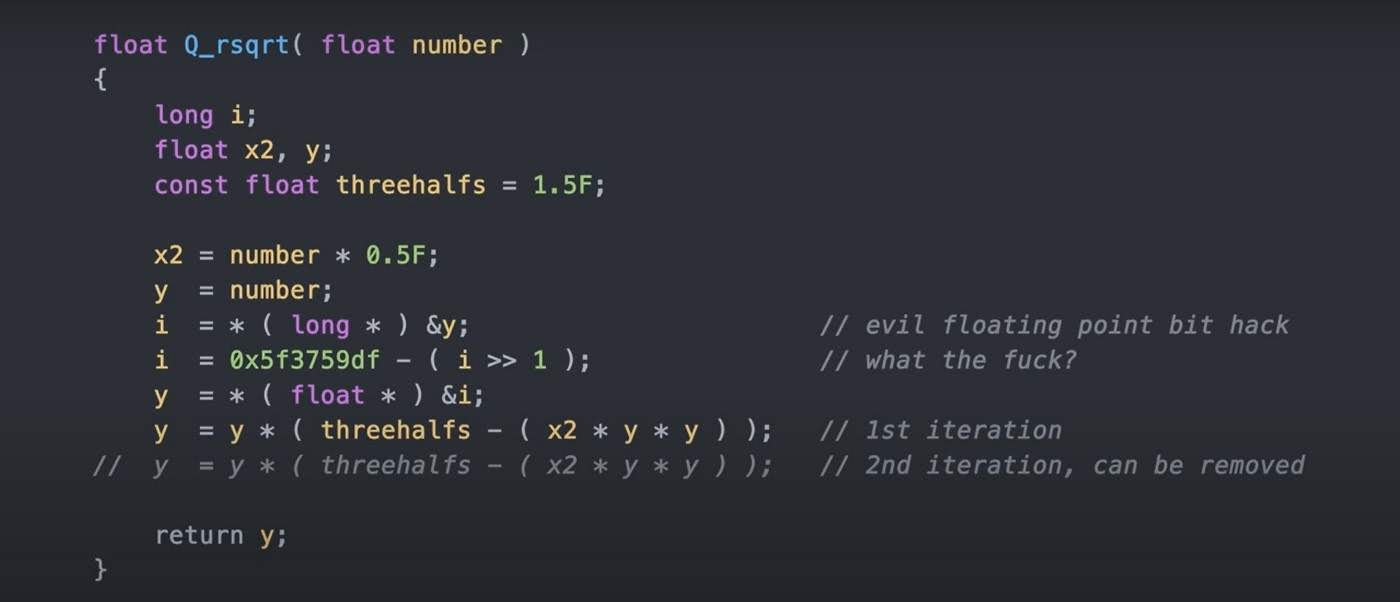
\includegraphics[interpolate, width=0.95\textwidth]{Q_rsqrt}
  \caption{Quake III inverse square root}
  \label{fig:rsqrt}
\end{figure}

\section {Задание \textnumero 2}

\lipsum[1-2]\ldots

\chapter{Заключение}

\lipsum[3-4]

\nocite{*} % prints the entire bibliography without citing anything
\printbibliography[
  heading=bibintoc,
  title={СПИСОК ИСПОЛЬЗОВАННЫХ ИСТОЧНИКОВ},
]

\end{document}